\RequirePackage{fix-cm}
\documentclass[8pt]{extarticle}
\usepackage{graphicx,blindtext,amsthm,tikz,wrapfig,amssymb,amsmath,xcolor,siunitx,breqn,caption,cancel,esdiff,multicol,multicol,xparse,stmaryrd,hyperref} % Required for inserting images
\usepackage[a4paper,top=0.5cm, bottom=0.5cm, left=0.5cm, right=0.5cm]{geometry}
\usetikzlibrary{positioning, arrows.meta}

\setlength{\columnsep}{0.2cm}


\DeclareMathOperator{\di}{\;d\!}
\DeclareMathOperator{\sech}{sech}
\DeclareMathOperator{\cosech}{csch}
\DeclareMathOperator{\arsec}{arsec}
\DeclareMathOperator{\arcot}{arCot}
\DeclareMathOperator{\arcosech}{arCsc}
\DeclareMathOperator{\arcosh}{arCosh}
\DeclareMathOperator{\arsinh}{arsinh}
\DeclareMathOperator{\artanh}{artanh}
\DeclareMathOperator{\arsech}{arsech}
\DeclareMathOperator{\arcsch}{arCsch}
\DeclareMathOperator{\arcoth}{arCoth}

\setlength{\parindent}{0pt}
\setlength{\abovedisplayskip}{1pt}
\setlength{\belowdisplayskip}{1pt}
\setlength{\abovedisplayshortskip}{0pt}
\setlength{\belowdisplayshortskip}{1pt}
\setlength{\jot}{1pt}

\newsavebox{\fitdisplaybox}
\newcommand{\fitdisplay}[1]{%
  \par\vspace{-1pt}\noindent
  \sbox{\fitdisplaybox}{#1}%
  \makebox[\columnwidth][c]{%
    \ifdim\wd\fitdisplaybox>\columnwidth
      \resizebox{\columnwidth}{!}{#1}%
    \else
      \usebox{\fitdisplaybox}%
    \fi
  }%
  \par\vspace{-1pt}%
}

% ===== Custom theorem-like environments with decimal numbers =====
% Paste this whole block into your preamble.

\newcounter{customthm}   % internal counter for cross‑referencing
\makeatletter

% Helper: define a theorem-like environment.
% #1 = environment name (e.g. theorem)
% #2 = printed heading (e.g. Theorem)
% #3 = style: plain, definition, remark
\newcommand{\definetheorem}[3]{%
  \newenvironment{#1}[1]{%
    \refstepcounter{customthm}%           % unique internal label
    \renewcommand{\@currentlabel}{##1}%   % store the custom decimal number
    \par\noindent
    \ifx#3plain\relax
      \textbf{#2 ##1.}\ \itshape
    \else\ifx#3definition\relax
      \textbf{#2 ##1.}\ \normalfont
    \else\ifx#3remark\relax
      \textit{#2 ##1.}\ \normalfont
    \else
      \textbf{#2 ##1.}\ \normalfont
    \fi\fi\fi
    \ignorespaces
  }{%
    \par
  }%
}

\makeatother

% Now create the environments you asked for.
\definetheorem{theorem}{Theorem}{plain}
\definetheorem{lemma}{Lemma}{plain}
\definetheorem{proposition}{Proposition}{plain}
\definetheorem{corollary}{Corollary}{plain}
\definetheorem{definition}{Definition}{definition}
\definetheorem{remark}{Remark}{remark}

\newenvironment{example}{%
  \par\noindent
  \textbf{Example.}\ \normalfont
  \ignorespaces
}{%
  \par
}

\makeatletter
\renewenvironment{proof}[1][\proofname]{%
  \par%
  \pushQED{\qed}%
  \normalfont
  \topsep=2pt\partopsep=0pt\parsep=0pt\itemsep=0pt%
  \trivlist
  \item[\hskip\labelsep\itshape #1\@addpunct{.}]\ignorespaces
}{%
  \popQED\endtrivlist\@endpefalse
  \vspace{-1pt}%
}
\makeatother

\begin{document}
\fontsize{5}{6.2}\selectfont

    \begin{multicols*}{5}
    \raggedright

        {\centering\fontsize{6}{6.8}\selectfont\textbf{Proofs}\par}
        \vspace{2pt}
        
        \begin{theorem}{1.1}
            (The Division Theorem for \(\mathbb{Z}\)): \(a,b\in\mathbb{Z}\) with \(b>0\) \(\exists ! q,r\in\mathbb{Z}\) with \(0\le r<b\) s.t. \(a=bq+r\).
        \end{theorem}

        \begin{proof}
            (\textit{Existance}):
            Let \(R=\{a-bm:m\in\mathbb{Z} \;\&\; a-bm\ge0\}\),
            then as:
            if \(a\ge0\), \(a-b\cdot 0=a\ge0\) so \(a\in R\);
            if \(a<0\), \(a-b\cdot a=a(1-b)\ge0\) so \(a-b\cdot a\in R\),
            \(R\ne\varnothing\).
            Thus, take \(r=\min(R)\) \& so \(0\le r=a-bm\in R\) for some \(m\in\mathbb{Z}\),
            choose \(q=m\in\mathbb{Z}\).
            So by construction \(a=bq+r\).
            Note, \(r<b\) as were such not true then \(r>a-b(q+1)=r-b\in R\) but this contradicts \(r=\min(R)\), so we have \(0\le r<b\).
            (\textit{Uniqueness}):
            Suppose \(q,q',r,r'\in\mathbb{Z}\) with \(0\le r',r<b\) \& \(a=bq+r=bq'+r'\),
            also WLOG take \(r'\le r\).
            So with \(\frac{r-r'}b\in(-1,1)\), \& \(\frac{r-r'}b=\frac{a-bq-(a-bq')}b=q'-q\in\mathbb{Z}\),
            we have \(\frac{r-r'}b=0\) i.e. \(r=r'\).
            So \(q=\frac{a-r}b=\frac{a-r'}b=q'\).
        \end{proof}

        \textbf{Euclidian Algorithm:}

        Let \(a,b\in\mathbb{Z}^+\), apply Th\textsuperscript{m} 1.1, to give:

        \fitdisplay{\(\begin{aligned}
            a&=bq_1+r_1\\
            b&=r_1q_2+r_2\\
            r_1&=r_2q_3+r_3\\
            &\hspace{5pt}\vdots\\
            r_{n-1}&=r_nq_{n+1}\text{,}
        \end{aligned}\)}

        Here, \(\gcd(a,b)=r_n\).
        To prove this relation we show: \(G(r_{i},r_{i+1})=G(r_{i+1},r_{i+2})\), where \(G(a,b)=\{n\in\mathbb{Z}:n|a\;\&\;n|b\}\).

        \textbf{Reverse Euclid:}

        Given a completed algorithm we can obtain \(n,m\in\mathbb{Z}\) s.t. \(na+mb=\gcd(a,b)\) i.e. taking the end of a Euclidian algroithm:

        \fitdisplay{\(\begin{aligned}
            &\hspace{5pt}\vdots\\
            r_{n-3}&=r_{n-2}q_{n-1}+r_{n-1}\quad(1)\\
            r_{n-2}&=r_{n-1}q_{n}+r_{n}\quad(2)\\
            r_{n-1}&=r_{n}q_{n+1}
        \end{aligned}\)}

        we have:

        From (2) and (1):
        \vspace{-6pt}
        \[
        \begin{aligned}
            r_n&=r_{n-2}-r_{n-1}q_n\quad(3)\\
            r_{n-1}&=r_{n-3}-r_{n-2}q_{n-1}\quad(4)
        \end{aligned}
        \]
        \vspace{-8pt}

        From (3) and (4):
        \vspace{-6pt}
        \[
        \begin{aligned}
            r_n&=r_{n-2}-r_{n-1}q_n\\
            &=r_{n-2}\\
            &\quad -(r_{n-3}-r_{n-2}q_{n-1})q_n\\
            &\hspace{5pt}\vdots
        \end{aligned}
        \]
        \vspace{-8pt}

        we continue this ladder up, simplifying each time,
        {\footnotesize (Note: \(r_{n}=\gcd(a,b)\))}

        \begin{theorem}{1.9}
            Every integer \(n\ge2\) can be written as a product of primes.
        \end{theorem}

        \begin{proof}
            (\textit{By strong induction}):

            (\textit{Base case}, \(n=2\)): Trivially true, \(n=2\) a product of primes.

            (\textit{Inductive Hypothesis}): Suppose for \(n\in{2,3,\ldots,k}\) \(n=p_{n,1}p_{n,2}\cdots p_{n,m_n}\).
            
            Then for \(n=k+1\), if \(k+1\) is prime we are done. If not, \(k+1=ab\) where \(a,b\in\{2,3,\ldots,k\}\), so by the hypothesis \(a\) and \(b\) are products of primes; hence \(k+1\) is too.

            So \(\forall n\in\mathbb{N}\) with \(n\ge2\), we are done.

        \end{proof}

        \begin{theorem}{1.10}
            (Euclid's property of primes) \(\forall p\in \text{Primes}\) \& \(\forall a,b\in\mathbb{Z}\). \(p|ab\implies p|a\text{ or } p|b\).
        \end{theorem}

        \begin{proof}
            (\textit{Case \(p|a\)}): We are done.

            (\textit{Case \(p\nmid a\)}): Then using the Euclidian algorithm we obtain: \(1=na-mp\) with \(n,m\in\mathbb{Z}\).
            So \(p|b\Longleftrightarrow p|(na-mp)b\Longleftrightarrow p|n(ab)-mbp\impliedby p|ab\).
        \end{proof}

        {\footnotesize the chain of implications uses a proposition in the notes which states: \(p|a\;\&\;p|b\implies p|a+b\;\&\;p|ab\)}.

        \begin{theorem}{1.12}
            (Fundamental Theorem of Arithmetic) \(\forall n\in\mathbb{N}\) with \(n\ge2\), \(\exists! p_1,p_2,\ldots,p_r\in\text{Primes}\) up to ordering, s.t.: \(n=p_1p_2\cdots p_r\).
        \end{theorem}

        \begin{proof}
            The existance is from Th\textsuperscript{m} 1.9. For uniqueness, suppose \(p_1p_2\cdots p_r=q_1q_2\cdots q_s\), then cancel common primes, suppose the result is not \(1\) i.e. we are left with \(p_1p_2\cdots p_n=q_1q_2\cdots q_m\) with \(p_i\ne q_j\),\(\forall i\in\{1,\ldots,n\}\) \& \(\forall j\in\{1,\ldots,m\}\), after reindexing. Then \(p_1|q_1q_2\cdots q_m\) so \(\exists j\in\{1,\ldots,m\}\)\(p_1|q_j\), but \(q_j\) is prime so \(p_1=q_j\), \(\lightning\).
        \end{proof}

        \begin{lemma}{1.16}
            \(\forall a,b\in R\): \(0a=a0=0\); \(a(-b)=(-a)b=-(ab)\); \& \((-a)(-b)=ab\)
        \end{lemma}

        \begin{proof}
            \(0a+0=0a=(0+0)a=0a+0a\) so \(0a=0\).
            
            \(ab+a(-b)=a(b-b)=a0=0=(a-a)b=ab+(-a)b\) so by the Groups \& Geo\textsuperscript{m} we have \(-(ab)\) is the unique element s.t. \(ab-(ab)=0\), \(a(-b)=-(ab)=(-a)b\).

            \((-a)(-b)=-(a(-b))=-(-(ab))=ab\).
        \end{proof}

        \begin{lemma}{1.18}
            (Subring Test) Let \(R\) be a ring \& \(S\subseteq R\). Then \(S\) is a subring of \(R\) iff the following hold, \(\forall r,s\in S\):

            \vspace{-10pt}
            \begin{enumerate}
                \item \(1_R\in S\),
                \vspace{-10pt}
                \item \(r+s,rs\in S\), \& 
                \vspace{-10pt}
                \item \(-r\in S\).
            \end{enumerate}
            \vspace{-10pt}
        \end{lemma}

        \begin{proof}
            By 1 \& 3 we have \(-1_R\in S\) so \(0_R=1_R-1_R\in S\) by 2. So \((S,+)\) is a group by the subgroup test with \((R,+)\).
            Commutativity of \(+\), associativity of \(+\) \& \(\times\), \& distributivity of \(\times\) over \(+\) are all inheritited from \(R\).
            Note, as they shair operations they shair the identities of the operations, so as, \(0_R\ne1_R\) in \(R\) we have \(0_S=0_R\ne 1_R=1_S\) in \(S\), so (R1)-(R4) are satisfied.
        \end{proof}

        \begin{lemma}{2.2}
            Suppose \(Char(R)=n>0\), then: (i) \(n\cdot r=0, \forall r\in R\); \& (ii) if \(m\in\mathbb{Z}^+\) then \(m\cdot 1=0\) iff \(n|m\).
        \end{lemma}
        

        \begin{proof}
            (i):

            \fitdisplay{\(\begin{aligned}
                n\cdot r&=\underbrace{r+r+\cdots+r}_{n\text{ times}}\\
                &=r(\underbrace{1+1+\cdots+1}_{n\text{ times}})=r0=0
            \end{aligned}\)}

            (ii): (\(\implies\)): Let \(m\cdot 1=0\) with \(m\in\mathbb{Z}^+\), applying the division Th\textsubscript{m} with \(m=nq+r\) where \(q,r\in\mathbb{Z}\) \& \(0\le r<n\) so \(0=m\cdot1=(nq+r)\cdot1=q(n\cdot1)+r\cdot1=q\cdot0+r\cdot1=r\cdot1\), so \(r=0\) as otherwise \(n>r\in\mathbb{Z}^+\) \& \(r\cdot 1=0\), a \(\lightning\) of \(n\)'s def\textsuperscript{n}.

            (\(\impliedby\)): Let \(n|m\) i.e. \(\exists q\in\mathbb{Z}\) s.t. \(m=qn\), so \(m\cdot1=qn\cdot1=q(n\cdot1)=q\cdot0=0\).
        \end{proof}


        \begin{lemma}{2.5}
            If \(S\) is a subring of \(R\) \& \(R\) is a domain then \(S\) is a domain.
        \end{lemma}

        \begin{proof}
            Let \(r,s\in S\) with \(rs=0\), thus \(rs=0\) in \(R\), hence \(r=0\) or \(s=0\).
        \end{proof}

        \begin{proposition}{2.7}
            Suppose \(R\) is a domain. Then \(R[X]\) is a domain.
        \end{proposition}

        \begin{proof}
            We use the contrapositive of the definition of a domain [i.e.:\(R\) a domain iff \(\forall 0\ne r,s\in R, rs\ne 0\)]. Let \(0\ne f,g\in R[X]\), taking the leading coefficients of \(f\) \& \(g\) as \(a\ne0\) \& \(b\ne0\), respectively, the leading coefficent of \(fg\) as \(ab\ne0\), hence \(fg\ne0\).
        \end{proof}

        {\footnotesize Note: This immediately (by induction on \(n\)) yields \(R[X_1,\ldots,X_n]\) is a domain if \(R\) is a domain.}

        \begin{lemma}{2.11}
            If \(R\) is a ring \& \(r\in R\) has both a left \& right inverse then these equal \& unique.
        \end{lemma}

        \begin{proof}
            (Equal): Choose, \(rs=1=tr\), then: \(s=1s=trs=t1=t\).

            (Unique right inverse): Let \(rs=1=rs'\) then \(s=1s=trs=t1=trs'=1s'=s'\), where t is choosen s.t. \(tr=1\).

            (Unique left inverse): Let \(tr=1=t'r\) then \(t=t1=trs=1s=t'rs=t'1=t'\), where s is choosen s.t. \(rs=1\)
        \end{proof}

        \begin{proposition}{2.13}
            Every division ring is a domain (\& subsequently every field is an integral domain).
        \end{proposition}

        \begin{proof}
            Let \(R\) be a division ring \& suppose \(r,s\in R\) \& \(rs=0\). Then assume \(r\ne0\) so \(r^{-1}\) exists, then \(s=r^{-1}rs=r^{-1}0=0\). Then given the immediate other case of \(r=0\) in all cases either \(r=0\) or \(s=0\). Hence \(R\) is a domain.
        \end{proof}

        \begin{lemma}{2.12}
            The following conditions for an integer \(n\ge2\) are equivalent:

            (i) \(\mathbb{Z}_n\) is an integral domain;\\
            (ii) \(\mathbb{Z}_n\) is a field;\\
            (iii) \(n\) is prime.
        \end{lemma}

        \begin{proof}
            (i)\(\implies\)(ii):
            Suppose \(\mathbb{Z}_n\) is a domain \& let \([m]_n\in\mathbb{Z}_n\) \& \([m]_n\ne0\). Consider the list \([0]_n[m]_n,[1]_n[m]_n,\ldots,[n-1]_n[m]_n\), each element in the list is distinct as, suppose otherwise then \([i]_n[m]_n=[j]_n[m]_n\) for some distinct \(i,j\in\{0,1,\ldots,n-1\}\), then \(([i]_n-[j]_n)[m]_n=0\) but \(\mathbb{Z}_n\) is suppose to be a domain \& \([m]_n\ne0\) so \([i]_n-[j]_n=[0]_n\) i.e. \([i]_n=[j]_n\), \(\lightning\). Then as there are \(n\) elements of the list each in \(\mathbb{Z}_n\), then \(\{[0m]_n,[1m]_n,\ldots,[(n-1)m]_n\}=\mathbb{Z}_n\). So some multiple of \([m]_n\) say \([r]_n\in\mathbb{Z}_n\) is s.t. \([m]_n[r]_n=[r]_n[m]_n=[1]_n\).

            (ii)\(\implies\)(iii):
            Suppose \(\mathbb{Z}_n\) is a field then suppose \(m,l\in\mathbb{N}\) are s.t. \(ml=n\), so \(0<m\le l\le n\). Then \([m]_n[l]_n=[ml]_n=[n]_n=[0]_n\) so as fields are domains, \([m]_n=[0]_n=[n]_n\) or \([l]_n=[0]_n=[n]_n\) \& so, by the equivalence class definition, \(m=n\) or \(l=n\) as neither are \(0\). So if \(m=n\), \(l=1\) \& if \(l=n\), \(m=1\), so the only factors of \(n\) are \(1\) \& \(n\) in \(\mathbb{N}\), i.e. \(n\) is prime.

            (iii)\(\implies\)(i):
            Suppose \(n\) is prime \& let \([m]_n,[l]_n\in\mathbb{Z}_n\) s.t. \([m]_n[l]_n=0\) i.e. \([ml]_n=[0]\) defintionally \(n\mid ml\) so by Th\textsuperscript{m} 1.10 \(n\mid m\) or \(n\mid l\) i.e. \([m]_n=[0]_n\) or \([l]_n=[0]_n\). So with \(\mathbb{Z}_n\)'s commutativity, \(\mathbb{Z}_n\) is an integral domain.
        \end{proof}

        \begin{proposition}{T1}
            In a domain \(R\) if \(ab=ac\) or \(ba=ca\) for \(a,b,c\in R\) \& \(a\ne0\) then \(b=c\).
        \end{proposition}

        \begin{proof}
            If \(ab=ac\), then \(a(b-c)=0\). If \(ba=ca\), then \((b-c)a=0\). Since \(a\ne0\) and \(R\) is a domain, \(b-c=0\).        
        \end{proof}

        \begin{lemma}{2.15}
            In a ring \(R\), the set of units \(R^*\) forms a group under multiplication.
        \end{lemma}

        \begin{proof}
            (G0): \(1\cdot1=1\) so \(1\in R^*\) i.e. \(R^*\ne\varnothing\); (G1): given (R2) we have associativity \& given \(r,s\in R^*\), \((rs)(s^{-1}r^{-1})=r(ss^{-1})r^{-1}=1\) \&
            \((s^{-1}r^{-1})(rs)=s^{-1}(r^{-1}r)s=1\), so \(rs\in R^*\) as required; (G2): (R4); \& (G3): Let \(r\in R^*\) so \(r\) is a unit so \(r^{-1}\in R^*\) exists, which itself has inverse \((r^{-1})^{-1}=r\in R\), so \(r^{-1}\in R^*\), as required.

        \end{proof}

        \vspace{-2pt}
        \noindent\makebox[\columnwidth][c]{%
            \resizebox{\columnwidth}{!}{%
            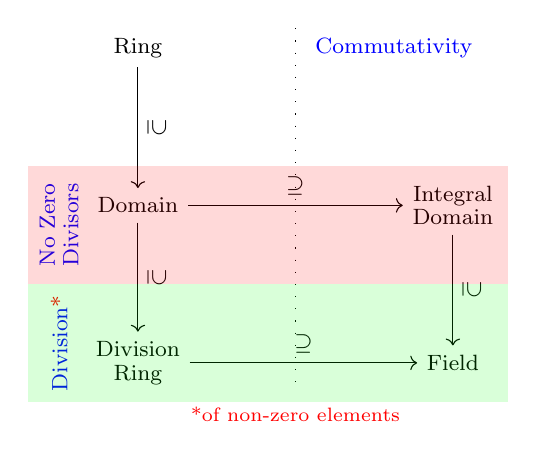
\begin{tikzpicture}[font=\fontsize{8}{8.5}\selectfont]
                \node (Ring) at (0,0) {Ring};
                \node (Domain) at (0,-2){Domain};
                \node[align=center] (Integral Domain) at (4,-2) {Integral\\ Domain};
                \node[align=center] (Division Ring) at (0,-4) {Division\\ Ring};
                \node (Field) at (4,-4) {Field};
                \node (Commutativity) at (3.25,0) {\textcolor{blue}{Commutativity}};
                \node[text=blue, align=center, rotate=90] (No Zero Divisors) at (-1,-2.25) {No Zero\\ Divisors};
                \node[text=blue, align=center, rotate=90] (Division*) at (-1,-3.75) {Division\textcolor{red}{*}};
                \node[text=red] (*of non-zero elements) at (2,-4.65) {{\fontsize{7}{7.5}\selectfont*of non-zero elements}};

                \draw[->] (Ring) -- (Domain) node[midway, above, sloped] {\(\supseteq\)};
                \draw[->] (Domain) -- (Integral Domain) node[midway, above, sloped] {\(\supseteq\)};
                \draw[->] (Domain) -- (Division Ring) node[midway, above, sloped] {\(\supseteq\)};
                \draw[->] (Division Ring) -- (Field) node[midway, above, sloped] {\(\supseteq\)};
                \draw[->] (Integral Domain) -- (Field) node[midway, above, sloped] {\(\supseteq\)};

                \draw[loosely dotted] (2,0.25) -- (2,-4.25);
                \fill[red, opacity=0.15] (-1.4,-1.5) rectangle (4.7,-3);
                \fill[green, opacity=0.15] (-1.4,-3) rectangle (4.7,-4.5);
                
            \end{tikzpicture}
            }
        }
        \vspace{-1pt}

        \begin{lemma}{3.3}
            Suppose \(\phi:R\to S\) is an isomorphism. Then: (i) \(\phi(1_R)=1_S\); (ii) \(\phi(0_R)=0_S\); (iii) \(\phi(-r)=-\phi(r)\), \(\forall r\in R\); (iv) \(r\in R\) is invertible iff \(\phi(r)\in S\) is invertible and, in that case, \((\phi(r))^{-1}=\phi(r^{-1})\); (v) \(r\in R\) is nilpotent iff \(\phi(r)\) is nilpotent and, in that case, they have the same index of nilpotence.
        \end{lemma}

        \begin{proof}
            (i): Let \(s\in S\). Since \(\phi\) is bijective, \(s=\phi(r)\) for some \(r\in R\). Then \(\phi(1_R)s=\phi(1_R)\phi(r)=\phi(r)=s\) and similarly \(s\phi(1_R)=s\), hence \(\phi(1_R)=1_S\).

            (ii): \(\phi(0_R)+1_S=\phi(0_R)+\phi(1_R)=\phi(1_R)=1_S\), so \(\phi(0_R)=0_S\).

            (iii): \(\phi(-r)+\phi(r)=\phi(0_R)=0_S\), so \(\phi(-r)=-\phi(r)\).

            (iv): If \(r\) is invertible then \(\phi(r^{-1})\phi(r)=\phi(r^{-1}r)=1_S\) and \(\phi(r)\phi(r^{-1})=\phi(rr^{-1})=1_S\), so \(\phi(r)\) is invertible with \((\phi(r))^{-1}=\phi(r^{-1})\). Conversely, apply this to \(\phi^{-1}:S\to R\).

            (v): Since \((\phi(r))^n=\phi(r^n)\), \(r^n=0_R\) iff \((\phi(r))^n=0_S\). Thus the least such \(n\) is the same.
        \end{proof}

        \begin{lemma}{3.7}
            Suppose \(\vartheta:R\to S\) is a homomorphism. Then: (i) \(\vartheta(0)=0\); (ii) \(\vartheta(-r)=-\vartheta(r)\), \(\forall r\in R\); (iii) if \(r\in R\) is invertible, then \(\vartheta(r)\in S\) is invertible and \((\vartheta(r))^{-1}=\vartheta(r^{-1})\); (iv) if \(r\in R\) is nilpotent, then \(\vartheta(r)\) is nilpotent with index \(\le\) the index of \(r\); (v) \(\operatorname{Im}(\vartheta)\) is a subring of \(S\).
        \end{lemma}

        \begin{proof}
            (i): As in Le\textsuperscript{m} 3.3(ii). (ii): As in Le\textsuperscript{m} 3.3(iii). (iii): If \(r\) is invertible then \(\vartheta(r^{-1})\vartheta(r)=\vartheta(r^{-1}r)=1_S\) and similarly \(\vartheta(r)\vartheta(r^{-1})=1_S\), so \((\vartheta(r))^{-1}=\vartheta(r^{-1})\). (iv): If \(r\) is nilpotent of index \(n\), then \(\vartheta(r)^n=\vartheta(r^n)=\vartheta(0)=0\), so \(\vartheta(r)\) has index at most \(n\). (v): Since \(\vartheta(1_R)=1_S\), \(1_S\in\operatorname{Im}(\vartheta)\). Let \(s=\vartheta(r)\), \(s'=\vartheta(r')\in\operatorname{Im}(\vartheta)\). Then \(s+s'=\vartheta(r+r')\), \(ss'=\vartheta(rr')\), and \(-s=-\vartheta(r)=\vartheta(-r)\), so by Le\textsuperscript{m} 1.18, \(\operatorname{Im}(\vartheta)\) is a subring of \(S\).
        \end{proof}

        \begin{lemma}{3.10}
            (i) If \(\vartheta:R\to S\) \& \(\beta:S\to T\) are homomorphisms then \(\beta\circ\vartheta:R\to T\) is a homomorphism. (ii) If \(\vartheta,\beta\) are embeddings then \(\beta\circ\vartheta\) is an embedding. (iii) If \(\vartheta,\beta\) are homomorphisms and \(\beta\circ\vartheta\) is an embedding then \(\vartheta\) is an embedding.
        \end{lemma}

        \begin{proof}
            (i): Let \(r,r'\in R\). Then
            \fitdisplay{\(\begin{aligned}
                \beta\circ\vartheta(r+r')&=\beta(\vartheta(r+r'))\\
                &=\beta(\vartheta(r)+\vartheta(r'))\\
                &=\beta\circ\vartheta(r)+\beta\circ\vartheta(r')
            \end{aligned}\)}
            Similarly, \(\beta\circ\vartheta(rr')=\beta\circ\vartheta(r)\beta\circ\vartheta(r')\), and
            \fitdisplay{\(\beta\circ\vartheta(1_R)=\beta(\vartheta(1_R))=\beta(1_S)=1_T\)}
            hence \(\beta\circ\vartheta\) is a homomorphism. (ii) \& (iii): follow from properties of injective maps.
        \end{proof}

        \begin{lemma}{3.15}
            If \(\vartheta: R\to S\) is a homomorphism then \(\vartheta\) is injective iff \(\text{ker}(\vartheta)={0}\).
        \end{lemma}

        \begin{proof}
            (\(\implies\)) Suppose \(\vartheta\) is injective. Then \(\vartheta(0)=0\) by le\textsuperscript{m} 3.7(i), then let \(r\in\text{ker}(\vartheta)\) then \(\vartheta(r)=0=\vartheta(0)\) so \(r=0\in\{0\}\), thus \(\text{ker}(\vartheta)={0}\).

            (\(\impliedby\)) Suppose \(\text{ker}(\vartheta)={0}\). Now let \(r,r'\in R\) s.t. \(\vartheta(r)=\vartheta(r')\) thus \(\vartheta(r-r')=\vartheta(r)-\vartheta(r')=0\) i.e. \(r-r'\in\text{ker}(\vartheta)=\{0\}\) so \(r-r'=0\), thus \(r=r'\), as required.
        \end{proof}

        \begin{lemma}{3.17}
            (i) Suppose \(\vartheta:R\to S\) is a homomorphism. Then \(\ker(\vartheta)\) is a subgroup of \((R,+)\). (ii) Let \(r,r'\in R\). Then \(\vartheta(r)=\vartheta(r')\) iff \(r-r'\in\ker(\vartheta)\) iff \(r\) \& \(r'\) belong to the same coset of \(\ker(\vartheta)\) in \(R\).
        \end{lemma}

        \begin{proof}
            (i): \(0\in\ker(\vartheta)\) so it is non-empty. Let \(r,r'\in\ker(\vartheta)\). Then \(\vartheta(r+r')=\vartheta(r)+\vartheta(r')=0+0=0\), so \(r+r'\in\ker(\vartheta)\). Also \(\vartheta(-r)=-\vartheta(r)=0\), so \(-r\in\ker(\vartheta)\). Hence by the subgroup test, \(\ker(\vartheta)\le(R,+)\). (ii): Let \(r,r'\in R\). Then
            \fitdisplay{\(\vartheta(r)=\vartheta(r')\Leftrightarrow\vartheta(r-r')=0\Leftrightarrow r-r'\in\ker(\vartheta)\)}
            \(\Leftrightarrow r+\ker(\vartheta)=r'+\ker(\vartheta)\).
        \end{proof}

        \begin{proposition}{3.22}
            A commutative ring \(R\) is a field iff the only ideals of \(R\) are \(R\) and \(\{0\}\).
        \end{proposition}

        \begin{proof}
            (\(\implies\)) Suppose \(R\) is a field, then clearly \(\{0\}\lhd R\) now suppose \(\{0\}\ne I\lhd R\) so then by defintion \(I\) contains a non-zero element of \(R\) say \(r\in I\). Now let \(s\in R\), so, as \(R\) is a field \(r^{-1}\) exists, then \(s=(sr^{-1})r\in I\), hence \(I=R\), as requried.
            (\(\impliedby\)) Suppose the only ideals of \(R\) are \(R\) and \(\{0\}\). Now let \(r\in R\setminus\{0\}\) then \(\langle r\rangle=R\) hence \(1\in\langle r\rangle\) so by the defintion of the principle ideal in a commutative ring \(1=sr(=rs)\) for some \(s\in R\), hence \(s\) is \(r\)'s inverse all non-zero elements in \(R\) have inverses, hence \(R\) is a field.
        \end{proof}

        \begin{proposition}{3.24}
            If \(\vartheta:R\to S\) is a homomorphism of rings, then \(\ker(\vartheta)\) is an ideal of \(R\).
        \end{proposition}

        \begin{proof}
            We show \(\ker(\vartheta)\) satisfies the three conditions for an ideal. Firstly \(0\in\ker(\vartheta)\). Let \(r,r'\in\ker(\vartheta)\). Then \(\vartheta(r+r')=\vartheta(r)+\vartheta(r')=0+0=0\), so \(r+r'\in\ker(\vartheta)\). Let \(s\in R\). Then \(\vartheta(sr)=\vartheta(s)\vartheta(r)=\vartheta(s)0=0\) and similarly \(\vartheta(rs)=0\). Therefore \(sr,rs\in\ker(\vartheta)\).
        \end{proof}

        \begin{corollary}{3.25}
            If \(\vartheta:R\to S\) is a homomorphism of rings and \(R\) is a field then \(\vartheta\) is a monomorphism.
        \end{corollary}

        \begin{proof}
            By Pro\textsuperscript{p} 3.24, \(\ker(\vartheta)\lhd R\), and so Pro\textsuperscript{p} 3.22 implies \(\ker(\vartheta)=\{0\}\) or \(R\). We cannot have \(\ker(\vartheta)=R\), as then \(1=\vartheta(1)=0\). Therefore \(\ker(\vartheta)=\{0\}\) and \(\vartheta\) is a monomorphism.
        \end{proof}

        \begin{proposition}{3.26}
            Suppose \(I\) and \(J\) are ideals of the ring \(R\). Then: (i) \(I+J=\{a+b:a\in I,b\in J\}\) is an ideal; (ii) \(I\cap J\) is an ideal; (iii) if \(\{I_\lambda\}_\lambda\) is any collection of ideals of \(R\), then \(\bigcap_\lambda I_\lambda\) is an ideal.
        \end{proposition}

        \begin{proof}
            (i): \(0\in I+J\), since \(0\in I\) and \(0\in J\). Let \(c,c'\in I+J\), say \(c=a+b\), \(c'=a'+b'\), for \(a,a'\in I\), \(b,b'\in J\). Then
            \fitdisplay{\(c+c'=(a+b)+(a'+b')=(a+a')+(b+b')\in I+J.\)}
            If \(r\in R\), then \(rc=r(a+b)=ra+rb\in I+J\) and similarly \(cr\in I+J\). Therefore \(I+J\lhd R\).

            (iii): Let \(K=\bigcap_\lambda I_\lambda\). Since \(0\in I_\lambda\) for every \(\lambda\), \(0\in K\). Let \(a,b\in K\). Then \(a,b\in I_\lambda\) for every \(\lambda\), so \(a+b\in I_\lambda\) for every \(\lambda\), hence \(a+b\in K\). If \(r\in R\), then \(ra,ar\in I_\lambda\) for every \(\lambda\), hence \(ra,ar\in K\). Thus \(K\lhd R\). (ii): This is the special case of (iii) with the collection \(\{I,J\}\).
        \end{proof}

        \begin{lemma}{4.2}
            (i) The operations \(+\) and \(\times\) on \(R/I\) are well-defined, i.e. if \(r+I=r'+I\) and \(s+I=s'+I\), then \((r+s)+I=(r'+s')+I\) and \(rs+I=r's'+I\). (ii) With these operations, \(R/I\) forms a ring. The zero element is \(0+I(=I)\), the identity is \(1+I\), and \(-(r+I)=(-r)+I\). If \(r^{-1}\) exists in \(R\), then \(r+I\) is invertible in \(R/I\) with inverse \(r^{-1}+I\).
        \end{lemma}

        \begin{proof}
            (i): Let \(r+I=r'+I\) and \(s+I=s'+I\), so \(r-r',s-s'\in I\). Then \((r-r')+(s-s')=(r+s)-(r'+s')\in I\), hence \((r+s)+I=(r'+s')+I\). Also \((r-r')s\in I\) and \(r'(s-s')\in I\), so \(rs-r's'=(r-r')s+r'(s-s')\in I\), hence \(rs+I=r's'+I\).

            (ii): By definition of \(+\) and \(\times\), \((r+I)+(0+I)=r+I\) and \((r+I)(1+I)=(1+I)(r+I)=r+I\). Associativity, distributivity, and commutativity of \(+\) are induced from \(R\). We have \((r+I)+((-r)+I)=0+I\), so \((R/I,+)\) is an abelian group. Finally, if \(r^{-1}\) exists in \(R\), then \((r+I)(r^{-1}+I)=1+I\) in \(R/I\).
        \end{proof}

        \begin{lemma}{4.4}
            Let \(I\) be a proper ideal of \(R\). (i) The map \(\pi:R\to R/I\), \(\pi(r)=r+I\), is a surjective ring homomorphism with kernel \(I\). (ii) Let \(\vartheta:R\to S\) be a homomorphism with \(I\subseteq\ker(\vartheta)\). There is an induced homomorphism \(\vartheta':R/I\to S\) with \(\vartheta'\circ\pi=\vartheta\).
        \end{lemma}

        \begin{proof}
            (i): Every element of \(R/I\) has form \(r+I=\pi(r)\), so \(\pi\) is surjective. Also \(\pi(r+s)=(r+s)+I=(r+I)+(s+I)=\pi(r)+\pi(s)\), similarly \(\pi(rs)=\pi(r)\pi(s)\), and \(\pi(1)=1+I\). Hence \(\pi\) is a homomorphism. Moreover
            \fitdisplay{\(\ker(\pi)=\{r\in R:\pi(r)=0+I\}=\{r\in R:r+I=I\}=I.\)}

            (ii): Define \(\vartheta':R/I\to S\) by \(\vartheta'(r+I)=\vartheta(r)\). If \(r+I=r'+I\), then \(r-r'\in I\subseteq\ker(\vartheta)\), so \(\vartheta(r-r')=0\), hence \(\vartheta(r)=\vartheta(r')\). Thus \(\vartheta'\) is well-defined. Also \(\vartheta'((r+I)+(s+I))=\vartheta'(r+s+I)=\vartheta(r+s)=\vartheta(r)+\vartheta(s)\), and similarly for multiplication, while \(\vartheta'(1+I)=1\). Thus \(\vartheta'\) is a homomorphism and \(\vartheta'\circ\pi=\vartheta\).
        \end{proof}

        \begin{theorem}{4.5}
            (Fundamental Isomorphism Theorem) Let \(\vartheta:R\to S\) be a ring homomorphism. Then \(R/\ker(\vartheta)\simeq\operatorname{Im}(\vartheta)\).
        \end{theorem}

        \begin{proof}
            Let \(I=\ker(\vartheta)\). By Lemma 4.4(ii), \(\vartheta':R/I\to S\) defined by \(\vartheta'(r+I)=\vartheta(r)\) is a homomorphism. We have \(\vartheta'(r+I)=0\) iff \(\vartheta(r)=0\) iff \(r\in\ker(\vartheta)=I\) iff \(r+I=0+I\), so \(\ker(\vartheta')=\{0+I\}\). By Lemma 3.15, \(\vartheta'\) is injective. Also \(\operatorname{Im}(\vartheta')=\operatorname{Im}(\vartheta)\). Therefore \(R/\ker(\vartheta)\simeq\operatorname{Im}(\vartheta)\).
        \end{proof}

        \begin{theorem}{4.8}
            Let \(I\) be a proper ideal of \(R\). Then ideals \(J\lhd R\) with \(J\ge I\) are in one-to-one correspondence with ideals \(K\lhd R/I\), via \(J\mapsto\pi J=\{\pi(r):r\in J\}\) and \(K\mapsto\pi^{-1}K=\{r\in R:\pi(r)\in K\}\).
        \end{theorem}

        \begin{proof}
            Let \(A=\{J\lhd R:J\ge I\}\) and \(B=\{K\lhd R/I\}\). Define \(f:A\to B\) by \(f(J)=\pi J\) and \(g:B\to A\) by \(g(K)=\pi^{-1}K\). First, to check these maps are well-defined, we check their outputs really lie in the stated codomains. If \(J\in A\), then \(\pi J\lhd R/I\), so \(f(J)\in B\): \(0=\pi(0)\in\pi J\); if \(b=\pi(a),b'=\pi(a')\in\pi J\), then \(b+b'=\pi(a+a')\in\pi J\); if \(s=\pi(r)\in R/I\), then \(bs=\pi(ar)\in\pi J\) and similarly \(sb\in\pi J\). If \(K\in B\), then \(\pi^{-1}K\lhd R\) and contains \(I\), so \(g(K)\in A\): \(0\in\pi^{-1}K\); if \(a,a'\in\pi^{-1}K\), then \(\pi(a+a')=\pi(a)+\pi(a')\in K\); and if \(r\in R\), then \(\pi(ar)=\pi(a)\pi(r)\in K\) and similarly \(\pi(ra)\in K\). Also \(I\subseteq\pi^{-1}K\), since \(a\in I\implies\pi(a)=0\in K\).

            Now \(g\) is the inverse of \(f\). For \(J\in A\), clearly \(J\subseteq\pi^{-1}(\pi J)\). Conversely, if \(a\in\pi^{-1}(\pi J)\), then \(\pi(a)=\pi(a')\) for some \(a'\in J\). Thus \(a-a'\in\ker(\pi)=I\subseteq J\), so \(a=a'+(a-a')\in J\). Hence \(\pi^{-1}(\pi J)=J\). For \(K\in B\), if \(b\in K\), surjectivity of \(\pi\) gives \(b=\pi(r)\), and \(r\in\pi^{-1}K\), so \(b\in\pi(\pi^{-1}K)\). Conversely, if \(b\in\pi(\pi^{-1}K)\), then \(b=\pi(r)\) for some \(r\in\pi^{-1}K\), hence \(b\in K\). Thus \(\pi(\pi^{-1}K)=K\). Therefore \(f\) and \(g\) are inverse bijections.
        \end{proof}

        \begin{theorem}{4.10}
            If \(I\le J\) are proper ideals of \(R\), so \(J/I\lhd R/I\), then \((R/I)/(J/I)\simeq R/J\).
            \begin{center}
                \vspace{-6pt}
                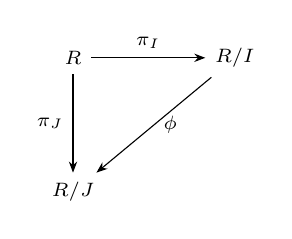
\begin{tikzpicture}[
                    font=\scriptsize,
                    node distance=1.25cm and 1.45cm,
                    >={Stealth[length=4pt]}
                ]
                    \node (R) {\(R\)};
                    \node[right=of R] (RI) {\(R/I\)};
                    \node[below=of R] (RJ) {\(R/J\)};
                    \draw[->] (R) -- node[above] {\(\pi_I\)} (RI);
                    \draw[->] (R) -- node[left] {\(\pi_J\)} (RJ);
                    \draw[->] (RI) -- node[right] {\(\phi\)} (RJ);
                \end{tikzpicture}
                \vspace{-12pt}
            \end{center}
        \end{theorem}

        \begin{proof}
            Use the Fundamental Isomorphism Theorem on \(\phi:R/I\to R/J\), \(\phi(r+I)=r+J\). This is a surjective homomorphism, and \(\ker(\phi)=\{r+I:r\in J\}=J/I\). Hence \((R/I)/(J/I)\simeq R/J\).
        \end{proof}

        \begin{corollary}{4.13}
            If \(R\) is commutative then a proper ideal \(I\lhd R\) is maximal iff the quotient ring \(R/I\) is a field.
        \end{corollary}

        \begin{proof}
            By Pro\textsuperscript{p} 3.22, it is enough to show \(I\) maximal iff the only ideals of \(R/I\) are \(\{0\}\) and \(R/I\). If \(I\) is maximal and \(K\lhd R/I\), then by Th\textsuperscript{m} 4.8, \(\pi^{-1}K\) is an ideal of \(R\) containing \(I\), so \(\pi^{-1}K=I\) or \(R\). Thus \(K=\{0\}\) or \(R/I\). Conversely, if \(R/I\) is a field and \(I\le J\lhd R\), then \(\pi J\lhd R/I\), so by Pro\textsuperscript{p} 3.22, \(\pi J=\{0\}\) or \(R/I\). By Th\textsuperscript{m} 4.8, this gives \(J=I\) or \(J=R\). Hence \(I\) is maximal.
        \end{proof}

        \begin{theorem}{4.16}
            Let \(I\) be a proper ideal of a commutative ring \(R\). Then \(I\) is prime iff \(R/I\) is an integral domain.
        \end{theorem}

        \begin{proof}
            Since \(R\) is commutative, so is \(R/I\), and since \(I\) is proper, \(0+I\ne1+I\). Suppose first that \(I\) is prime. If \((r+I)(s+I)=0+I\), then \(rs+I=0+I\), so \(rs\in I\). Hence \(r\in I\) or \(s\in I\), i.e. \(r+I=0+I\) or \(s+I=0+I\). Thus \(R/I\) has no zero divisors, so it is an integral domain.

            Conversely, suppose \(R/I\) is an integral domain. If \(rs\in I\), then \((r+I)(s+I)=rs+I=0+I\). Since \(R/I\) has no zero divisors, \(r+I=0+I\) or \(s+I=0+I\), so \(r\in I\) or \(s\in I\). Thus \(I\) is prime.
        \end{proof}

        \begin{theorem}{5.1}
            (Division Theorem for Polynomials) Let \(K\) be a field and \(f,g\in K[X]\) with \(g\ne0\). Then there are unique \(q,r\in K[X]\) with \(f=qg+r\) and \(\deg(r)<\deg(g)\) or \(r=0\).
        \end{theorem}

        \begin{proof}
            Let \(A=\{f-hg:h\in K[X]\}\). Choose \(r=f-qg\in A\) of least degree. If \(r=0\) or \(\deg(r)<\deg(g)\), done. Otherwise, since \(K\) is a field, a suitable scalar multiple of \(X^{\deg r-\deg g}g\) can be subtracted from \(r\) to cancel its leading term, giving \(r-hg=f-(q+h)g\in A\) of smaller degree, contradiction. For uniqueness, if \(qg+r=q'g+r'\), then \((q-q')g=r'-r\). If \(q\ne q'\), the left has degree at least \(\deg(g)\), while the right has degree \(<\deg(g)\), impossible. Thus \(q=q'\) and \(r=r'\).
        \end{proof}

        \begin{corollary}{5.4}
            Let \(K\) be a field, \(f\in K[X]\), and \(a\in K\). Then \(a\) is a root of \(f\) iff \(X-a\) is a factor of \(f\).
        \end{corollary}

        \begin{proof}
            If \(X-a\mid f\), then \(f(a)=0\). Conversely, suppose \(f(a)=0\). Divide \(f\) by \(X-a\): \(f=q(X-a)+r\), where \(r=0\) or \(\deg r<1\), so \(r\) is constant. Substituting \(X=a\) gives \(0=f(a)=r\). Hence \(f=q(X-a)\).
        \end{proof}

        \begin{corollary}{5.6}
            Let \(K\) be a field and \(f,g\in K[X]\). Then the ideal generated by \(f\) and \(g\) equals the ideal generated by their greatest common divisor, i.e. \(\langle f,g\rangle=\langle\gcd(f,g)\rangle\).
        \end{corollary}

        \begin{theorem}{5.8}
            Let \(K\) be a field. Then every ideal of \(K[X]\) is principal.
        \end{theorem}

        \begin{proof}
            Let \(I\lhd K[X]\). If \(I=\{0\}=\langle0\rangle\), then \(I\) is principal. Otherwise choose non-zero \(g\in I\) of least degree. Let \(f\in I\). By Theorem 5.1, \(f=qg+r\) with \(r=0\) or \(\deg(r)<\deg(g)\). Since \(r=f-qg\in I\), minimality of \(\deg(g)\) forces \(r=0\). Hence every \(f\in I\) is a multiple of \(g\), so \(I=\langle g\rangle\).
        \end{proof}

        \begin{lemma}{6.2}
            Let \(K\) be a field and \(f\in K[X]\) be irreducible. Then \(\langle f\rangle\) is a maximal ideal of \(K[X]\).
        \end{lemma}

        \begin{proof}
            Let \(\langle f\rangle\le I\le K[X]\). By Th\textsuperscript{m} 5.8, \(I=\langle g\rangle\). Since \(f\in\langle g\rangle\), \(f=qg\) for some \(q\in K[X]\). As \(f\) is irreducible, \(q\) or \(g\) is invertible. If \(q\) is invertible, then \(\langle g\rangle=\langle f\rangle\). If \(g\) is invertible, then \(\langle g\rangle=K[X]\). Hence \(\langle f\rangle\) is maximal.
        \end{proof}

        \begin{theorem}{6.3}
            (Kronecker's Theorem) Let \(K\) be a field and \(f\in K[X]\) be irreducible of degree \(n\). Define \(L=K[X]/\langle f\rangle\). Then: (i) \(L\) is a field and \(\pi:K[X]\to L\) induces an embedding \(\vartheta:K\to L\); (ii) \(\alpha=X+\langle f\rangle\) is a root of \(f\) in \(L\); (iii) \(L\) is a vector space over \(K\) of dimension \(n\), with basis \(\{1,\alpha,\ldots,\alpha^{n-1}\}\).
        \end{theorem}

        \begin{proof}
            (i): By Lemma 6.2, \(\langle f\rangle\) is maximal, so \(L\) is a field by Corollary 4.13. Define \(\vartheta:K\to L\) by \(\vartheta(a)=a+\langle f\rangle\). This is a homomorphism. If \(\vartheta(a)=\vartheta(b)\), then \(a-b\in\langle f\rangle\). Since \(\deg(f)\ge1\), this forces \(a-b=0\), so \(\vartheta\) is injective.

            (ii): Let \(f=b_0+b_1X+\cdots+b_nX^n\). For \(\alpha=X+\langle f\rangle\),
            \fitdisplay{\(f(\alpha)=b_0+b_1\alpha+\cdots+b_n\alpha^n=f+\langle f\rangle=\langle f\rangle=0_L.\)}
            Thus \(\alpha\) is a root of \(f\) in \(L\).

            (iii): If \(g+\langle f\rangle\in L\), divide \(g\) by \(f\): \(g=qf+r\), with \(r=0\) or \(\deg(r)<n\). Writing \(r=a_0+a_1X+\cdots+a_{n-1}X^{n-1}\), we get
            \fitdisplay{\(g+\langle f\rangle=r+\langle f\rangle=a_0+a_1\alpha+\cdots+a_{n-1}\alpha^{n-1}.\)}
            Thus \(L\) is spanned by \(1,\alpha,\ldots,\alpha^{n-1}\). Linear independence follows since any non-zero polynomial of degree \(<n\) cannot lie in \(\langle f\rangle\).
        \end{proof}

        \vspace{2pt}
        {\centering\fontsize{6}{6.8}\selectfont\textbf{Definitions}\par}
        \vspace{2pt}

        \begin{definition}{1.4}
            \(\forall a,b\in\mathbb{Z}\), \(\gcd(a,b)=\max\{n\in\mathbb{Z}:n|a\;\&\;n|b\}\), noting \(\gcd(0,0)=0\) \& if \(\gcd(a,b)=1\) then \(a\) \& \(b\) are coprime.
        \end{definition}

        \begin{definition}{1.6}
            \(\forall a,b,n\in\mathbb{Z}\) with \(n\ge2\).
            \(a\) is \textbf{congruent to} \(b\) \textbf{modulo} \(n\) iff \(n|a-b\), written \(a\equiv b\mod n\).Then define the congruence class of \(a\) w.r.t. \(n\) as: \([a]_n=\{b\in\mathbb{Z}:b\equiv a\mod n\}=\{b\in\mathbb{Z}:n\mid(b-a)\}=\{a+kn:k\in\mathbb{Z}\}\)
            
            We thus have: 
            
            \fitdisplay{\(\mathbb{Z}_n=\{[a]_n:a\in\mathbb{Z}\}=\{[0]_n,[1]_n,\ldots,[n-1]_n\}\)}

            {\footnotesize Note: \(b\equiv a \mod n\) iff \(b=a+kn\) iff \([a]_n=\{a+nk:k\in\mathbb{Z}\}\) iff \([a]_n=[a+kn]_n\)}
        \end{definition}

        \begin{definition}{1.14}
            A \textbf{ring} is a set \(R\) with two binary operations \(+\) \& \(\times\), defined on \(R\), satisfying the following:

            (R1) \((R,+)\) is an abelian group with identity 0.

            (R2) \(\times\) is associative.

            (R3) \(\times\) distributes over \(+\) i.e.:

            \fitdisplay{\(\begin{aligned}a(b+c)&=ab+ac,\\(a+b)c&=ac+bc,\quad \forall a,b,c\in R\end{aligned}\)}

            (R4) The multiplicative identity \(1\in R\) \& \(1\ne0\)


        \end{definition}

        \begin{example}
            With \(n\ge 2\), \(M_n(R)\) is the ring of \(n\times n\) matrices, a non-commutative ring.
            {\footnotesize Note: the only two-sided ideals of \(M_n(F)\), \(F\) a field, are \(M_n(F)\) \& \(\{\mathbf{0}\}\) but this isn't a division ring hence even relaxing commutative in Pro\textsuperscript{p} 3.22 doesn't yeild the same pro\textsuperscript{p} with field \(\to\) division ring.}
        \end{example}

        \begin{example}
            For \(X\) a set \(\mathcal{P}(X)\) with
            
            \fitdisplay{\(\begin{aligned}A+B&=(A\cup B)\setminus(A\cap B),\\ AB&=A\cap B\end{aligned}\)}

            \& \(0=\varnothing\), \(-A=A\), \(A,B\in\mathcal{P}(X)\).
        \end{example}

        \begin{definition}{1.17}
            Let \(R\) be a ring \& \(S\subseteq R\). Then \(S\) is a \textbf{subring} of \(R\) if \(S\) is a ring w.r.t. the same addition \& multiplication as \(R\) \& contains the multiplicative identity of \(R\), \(1_R\).
        \end{definition}

        \begin{definition}{1.21}
            let \(R\) be a ring. The \textbf{ring of polynomials} \(R[X]=\{\sum_{i\ge0}^na_iX^i\text{ a finite sum}:a_i\in R\}\) with addition \& multiplication defined as:
            
            \(\sum_{i\ge0}^na_iX^i+\sum_{i\ge0}^mb_iX^i=\sum_{i\ge0}^{\max(n,m)}(a_i+b_i)X^i\)
            
            \&
            
            \(\big(\sum\limits_{i\ge0}^na_iX^i)(\sum\limits_{i\ge0}^mb_iX^i)=\sum\limits_{i\ge0}^{n+m}(\sum\limits_{j=0}^ia_{j}b_{i-j})X^i\)
            {\footnotesize (taking missing coefficients as 0)}
            
            \(0=\sum_{i\ge0}0X^i\) \& \(1=1X^0+\sum_{i\ge1}0X^i\). Then the \textbf{degree} of a polynomial is the greatest \(i\in\mathbb{N}\cup\{0\}\) s.t. \(a_i\ne0\) or if no such \(i\) exist \(\deg(0)=-\infty\)

            More genearlly, we have:
            
            \fitdisplay{\(R[X_1,\ldots,X_n]=R[X_1,\ldots,X_{n-1}][X_n]\)}

            {\footnotesize \(\forall f,g\in R[X]\), \(\deg(f+g)\le\max(\deg(f),\deg(g))\)} \& \(\deg(fg)\le\deg(f)+\deg(g)\).
        \end{definition}

        \begin{definition}{1.24}
            If \(R_1\) \& \(R_2\) are rings then the \textbf{Cartesian product} \(R_1\times R_2\) with the \(+\) \& \(\times\) defined element wise is a ring.
        \end{definition}

        \begin{definition}{2.1}
            For \(a\in R\) define: for \(n\in\mathbb{Z}^+\), \(n\cdot a=\underbrace{a+a+\cdots+a}_{n\text{ times}}\); for \(n=0\), \(n\cdot a=0\cdot a=0\); \& for \(n\in\mathbb{Z}^-\), \(n\cdot a=(-n)\cdot(-a)\).
            
            The \textbf{Characteristic}, \(\text{char}(R)\), of a ring \(R\) is the least posititve integer \(n\) s.t. \(n\cdot 1=0\), or if no exist \(\text{char}(R)=0\).
            
            {\footnotesize Note: \((n+m)\cdot a=n\cdot a+m\cdot a\), \(n\cdot(a+b)=n\cdot a+n\cdot b\), \& \(n\cdot(m\cdot a)=(nm)\cdot a\), all easily verifiable.}
        \end{definition}

        \begin{definition}{2.3}
            A non-zero element \(r\in R\) is a \textbf{zero-divisor} if \(\exists s\in R\) a non-zero element s.t. \(rs=0\) or \(sr=0\).

            A ring \(R\) is a domain if, \(\forall r,s\in R\):

            \fitdisplay{\(rs=0\implies r=0 \text{ or } s=0.\)}

            i.e. a ring with no zero divisors is a domain \& vice versa.
        \end{definition}

        \begin{definition}{2.9}
            A \textbf{division ring} is a ring where every non-zero element has a right \& left inverse, i.e.: \(\forall r\in R\setminus\{0\},\exists s,t\in R\text{ s.t. }rs=1=tr\) with \(s\),\(t\) being the right \& left inverses, respectively.

            {\footnotesize Note: this immediately collapse, due to Le\textsuperscript{m} 2.11, to just there exists an inverse as \(s=t\).}
            
            An \textbf{invertible} element \(r\) is called a \textbf{unit}.
        \end{definition}

        \begin{example}
            Division rings are not all fields e.g. the quaternions \(\mathbb{H}=\{a+bi+cj+dk:a,b,c,d\in\mathbb{R}\}\) where \(i^2=j^2=k^2=-1\) \& \(ij=k\), \(jk=i\), \& \(ki=j\), this is non-commutative as \(-ij=-k=jjk=ji\) so \(ij\ne ji\) and this is a division ring as for \(z=a+bi+cj+dk\) \(z^{-1}=\frac{a-bi-cj-dk}{a^2+b^2+c^2+d^2}\), taking \(z\ne0\).
        \end{example}
       
        \begin{definition}{2.16}
            An element \(r\) of a ring \(R\) is \textbf{nilpotent} if \(\exists n\in\mathbb{Z}^+\) s.t. \(r^n=0\), and the least such \(n\) is the \textbf{index of nilpotence} of \(r\).

            An element \(r\in R\) is \textbf{idempotent} if \(r^2=r\).

            {\footnotesize Note: In any ring \(R\), \(0_R\) is nilpotent with index 1 and \(0_R\) and \(1_R\) are idempotent.}
        \end{definition}

        \begin{definition}{3.1}
            If \(R\) \& \(S\) are rings then an \textbf{isomorphism} from \(R\) to \(S\) is a bijection \(\phi:R\to S\) s.t. \(\forall r,r'\in R\):

            \fitdisplay{\(\begin{aligned}\phi(r+r')&=\phi(r)+\phi(r'),\\ \phi(rr')&=\phi(r)\phi(r')\end{aligned}\)}

            \(\exists\phi:R\to S\) an isomorphism iff \(R\) \& \(S\) are \textbf{isomorphic}, written \(R\simeq S\).
        \end{definition}

        \begin{example}
            For 4 element rings \(\mathbb{Z}_4 \not\simeq \mathbb{Z}_2\times\mathbb{Z}_2\), since given \([2]_4\ne0\) and \([2]_4^2=[0]_4\), \([2]_4\) is nilpotent, where as there are no non-zero nilpotent elements in \(\mathbb{Z}_2\times\mathbb{Z}_2\), hence the result by Le\textsuperscript{m} 3.3.
        \end{example}

        \begin{definition}{3.6}
            If \(R\) \& \(S\) are rings then a \textbf{homomorphism} from \(R\) to \(S\) is a map \(\vartheta:R\to S\) s.t. \(\forall r,r'\in R\):

            \fitdisplay{\(\begin{aligned}\vartheta(r+r')&=\vartheta(r)+\vartheta(r'),\\ \vartheta(rr')&=\vartheta(r)\vartheta(r'),\\ \vartheta(1_R)&=1_S.\end{aligned}\)}
        \end{definition}

        \begin{example}
            The map \(\mathbb{Z}\to\mathbb{Z}_n\) by \(m\mapsto[m]_n\) is a homomorphism. Also, \(\vartheta:\mathbb{Z}_{kn}\to\mathbb{Z}_n\) by \(\vartheta([m]_{kn})=[m]_n\) is a homomorphism, well definedness must be shown, and is true as; let \([m]_{kn}=[m']_{kn}\in\mathbb{Z}_{kn}\) then \(kn\mid m-m'\) so \(n|m-m'\) thus \([m]_n=[m']_{n}\).
        \end{example}

        \begin{definition}{3.9}
            An \textbf{embedding} or \textbf{monomorphism} is an injective homomorphism.
            {\footnotesize There is a trivial embedding along each arrow of \(\mathbb{Z}\to\mathbb{Q}\to\mathbb{R}\to\mathbb{C}\to\mathbb{C}[X].\)}
        \end{definition}

        \begin{example}
            With \(R\) a ring, the map \(R[X]\to R[X]\) by \(p(X)\mapsto p(q(X))\) for some \(q(X)\in R[X]\).
        \end{example}

        \begin{definition}{3.12}
            If \(\vartheta :R\to S\) is a ring homomorphism, then the \textbf{kernel} of \(\vartheta\) is defiend as \(\text{ker}(\vartheta)=\{r\in R:\vartheta(r)=0_S\}\).
        \end{definition}

        \begin{definition}{3.16}
            An \textbf{automorphism} of a ring is an isomorphism from and to itself.
        \end{definition}

        \begin{example}
            \(\mathbb{Z}[i]\to\mathbb{Z}[i]\) by \(a+bi\mapsto a-bi\) is an automorphism.
        \end{example}

        \begin{definition}{3.18}
            An \textbf{ideal} of a ring \(R\) is a subset \(I\subseteq R\) s.t.: \(0\in I\); \(a+b\in I\), \(\forall a,b\in I\); \& \(ar,ra\in I\), \(\forall a\in I\), \(\forall r\in R\). We write \(I\lhd R\) to mean \(I\) is an ideal of \(R\).
        \end{definition}

        \begin{definition}{3.19}
            If \(a\in R\) then \(\{r_1as_1+\cdots+r_nas_n:n\ge1,\;r_i,s_i\in R\}\) is an ideal containing \(a\) and is the smallest ideal of \(R\) containing \(a\). It is called the \textbf{principal ideal generated by} \(a\), denoted \(\langle a\rangle\). If \(R\) is commutative then \(\langle a\rangle=\{ar:r\in R\}\). A \textbf{principal ideal} is one which can be generated by a single element.
        \end{definition}

        \textbf{Examples 3.20.}
        (i) In every ring \(\langle0\rangle=\{0\}\) is the smallest ideal, the \textbf{trivial ideal}.
        (ii) In every ring \(\langle1\rangle=R\) is an ideal and every other ideal \(\ne R\) is a \textbf{proper ideal}.
        (iii) If \(n\in\mathbb{Z}\) then \(\langle n\rangle=\{nk:k\in\mathbb{Z}\}\).
        (iv) If \(p\in R[X]\) then \(\langle p\rangle\) is the set of polynomials with \(p\) as a factor.

        \begin{definition}{3.21}
            A \textbf{right ideal} is defined as for a general ideal but with the third condition replaced by the weaker condition: \(a\in I\) and \(r\in R\) implies \(ar\in I\). A \textbf{left ideal} is defined similarly. If \(a\in R\), the \textbf{principal right ideal generated by} \(a\) is \(\{ar:r\in R\}\), denoted \(aR\).
        \end{definition}

        \begin{example}
            Let \(R=M_2(\mathbb{Z})\) and \(A=\begin{pmatrix}1&0\\0&0\end{pmatrix}\) then by simple multiplication the principle left and right ideals are \(\{\begin{pmatrix}
                a&0\\b&0
            \end{pmatrix}:a,b\in \mathbb{Z}\}\) and \(\{\begin{pmatrix}
                a&b\\0&0
            \end{pmatrix}:a,b\in \mathbb{Z}\}\) whilst \(\langle A\rangle=M_2(\mathbb{Z})\) as \(I_2=A+\begin{pmatrix}0&1\\1&0\end{pmatrix}A\begin{pmatrix}0&1\\1&0\end{pmatrix}\in\langle A\rangle\)

            {\footnotesize Note: If \(1\in I\) with \(I\lhd R\) the \(\forall r \in R\) \(r=r1\in I\), so \(I=R\).}
        \end{example}

        \begin{definition}{3.22}
            Let \(A\subseteq R\) and \(R\) be a commutative ring, then \(\{a_1r_1+\cdots+a_nr_n:n\ge1,a_i\in A,r_i\in R\}\) is the \textbf{ideal generated by} \(A\).
        \end{definition}

        \begin{example}
            Working in \(\mathbb{Z}[X]\) the ideal \(I=\langle 2,X\rangle:=\langle \{2,X\}\rangle\) is not a principal ideal. Suppose \(I=\langle p\rangle\). Since \(2\in I\), \(2=pq\) for some \(q\in\mathbb{Z}[X]\). As \(\mathbb{Z}\) is a domain, \(0=\deg(2)=\deg(pq)=\deg(p)+\deg(q)\), so \(p,q\in\mathbb{Z}\) and \(p=\pm1\) or \(p=\pm2\). If \(p=\pm1\), then \(1=2r_1+Xr_2\) for some \(r_1,r_2\in\mathbb{Z}[X]\), impossible since the RHS has even constant term. Hence \(p=\pm2\). But \(X\in I\), so \(X=2r_3\) for some \(r_3\in\mathbb{Z}[X]\), impossible since \(2r_3\) has even coefficients. Thus \(I\) is not principal.
        \end{example}

        \begin{definition}{3.26}
            We can also define a \textbf{product of ideals}: if \(I,J\lhd R\), then their product is the ideal generated by \(\{ab:a\in I,b\in J\}\). This set will not in general be closed under addition, hence we say ``generated by''. Powers of an ideal are defined inductively by \(I^{n+1}=I^nI\).
        \end{definition}

        \begin{definition}{4.1}
            Let \(R\) be a ring and let \(I\) be a proper ideal. Let \(R/I\) denote the set of cosets of \(I\) in the additive group \((R,+)\):
            \fitdisplay{\(R/I=\{r+I:r\in R\}.\)}
            Define operations \(+\) and \(\times\) on \(R/I\) by
            \fitdisplay{\((r+I)+(s+I)=(r+s)+I,\quad (r+I)(s+I)=rs+I.\)}
        \end{definition}

        \begin{definition}{4.1}
            The ring \(R/I\) is called the \textbf{factor ring} (or \textbf{quotient ring}) of \(R\) by \(I\).
        \end{definition}

        \begin{example}
            \(\mathbb{Z}/\langle n\rangle=\mathbb{Z}_n\).
        \end{example}

        \textbf{Exercise.} Write out the elements of the factor ring \(\mathbb{Z}_6/\langle[3]_6\rangle\). What is this factor ring isomorphic to?

        \begin{definition}{4.4}
            The map \(\pi:R\to R/I\), \(\pi(r)=r+I\), is called the \textbf{canonical projection}, or \textbf{canonical surjection}.
        \end{definition}

        \begin{example}
            \textbf{4.6.} Take \(R=\mathbb{Z}\) and \(I=\langle6\rangle=6\mathbb{Z}\), so the canonical projection is \(\pi:\mathbb{Z}\to\mathbb{Z}_6\). Let \(\vartheta:\mathbb{Z}\to\mathbb{Z}/\langle2\rangle=\mathbb{Z}_2\) be the canonical projection. Then \(\ker(\vartheta)=\langle2\rangle\supseteq\langle6\rangle\), so by Le\textsuperscript{m} 4.4 there is a unique homomorphism \(\vartheta'\) with \(\vartheta'\circ\pi=\vartheta\). This is the map \(\vartheta':\mathbb{Z}_6\to\mathbb{Z}_2\) already seen in Examples 3.8.
        \end{example}

        \begin{example}
            \textbf{4.7.} Let \(R=\mathbb{R}[X]\) and \(I=\langle X^2+1\rangle\). Let \(\pi:\mathbb{R}[X]\to\mathbb{R}[X]/\langle X^2+1\rangle\) be the canonical surjection. Let \(\vartheta:\mathbb{R}[X]\to\mathbb{C}\) be evaluation at \(i\), \(\vartheta(p(X))=p(i)\). Then \(p\in\ker(\vartheta)\) iff \(X^2+1\mid p\), so \(\ker(\vartheta)=\langle X^2+1\rangle\). By Le\textsuperscript{m} 4.4, there is a unique map \(\vartheta':\mathbb{R}[X]/\langle X^2+1\rangle\to\mathbb{C}\) through which \(\vartheta\) factors. It is injective and surjective, hence an isomorphism. Thus \(\mathbb{R}[X]/\langle X^2+1\rangle\simeq\mathbb{C}\).
        \end{example}

        {\footnotesize Notation: if \(I\subseteq J\) are ideals then usually write \(I\le J\) (or \(J\ge I\)) instead of subset notation, with the same meaning.}

        \begin{example}
            \textbf{4.9.} The ideals of \(\mathbb{Z}_6=\mathbb{Z}/\langle6\rangle\) are in one-to-one correspondence with the ideals of \(\mathbb{Z}\) containing \(\langle6\rangle\). There are \(4\) of each: \(\langle1\rangle,\langle2\rangle,\langle3\rangle,\langle6\rangle\) correspond to
            \fitdisplay{\(\begin{aligned}
                \pi\langle1\rangle&=\mathbb{Z}_6=\{[0]_6,[1]_6,[2]_6,[3]_6,[4]_6,[5]_6\},\\
                \pi\langle2\rangle&=\langle[2]_6\rangle=\{[0]_6,[2]_6,[4]_6\},\\
                \pi\langle3\rangle&=\langle[3]_6\rangle=\{[0]_6,[3]_6\},\\
                \pi\langle6\rangle&=\langle[0]_6\rangle=\{[0]_6\}.
            \end{aligned}\)}
        \end{example}

        {\footnotesize The notation \(J/I\) is also used instead of \(\pi J\) for the image of \(J\) in \(R/I\).}

        \begin{example}
            \textbf{4.11.} Since \(\langle6\rangle\le\langle2\rangle\), Th\textsuperscript{m} 4.10 gives \((\mathbb{Z}/\langle6\rangle)/(\langle2\rangle/\langle6\rangle)\simeq\mathbb{Z}/\langle2\rangle\).
        \end{example}

        \begin{definition}{4.12}
            An ideal \(I\) of a ring \(R\) is \textbf{maximal} if it is proper and for any ideal \(J\) with \(I\le J\le R\), either \(J=I\) or \(J=R\).
        \end{definition}

        \begin{definition}{4.14}
            A proper ideal \(I\) of a commutative ring \(R\) is \textbf{prime} if whenever \(r,s\in R\) and \(rs\in I\), then \(r\in I\) or \(s\in I\).
        \end{definition}

        \begin{example}
            \textbf{4.15.} All ideals of \(\mathbb{Z}\) are principal. The prime ideals are precisely the ideals generated by a prime number or zero.
        \end{example}

        \begin{example}
            \textbf{5.2.} In \(\mathbb{Z}_5[X]\),
            \fitdisplay{\(X^4+2X^2+X+4=(X^2+2X+3)(X^2+3X+3)+X.\)}
        \end{example}

        \begin{definition}{5.3}
            An element \(a\in K\) is a \textbf{root} (or \textbf{zero}) of \(f\in K[X]\) iff \(f(a)=0\).
        \end{definition}

        \begin{definition}{5.5}
            The \textbf{greatest common divisor} of polynomials \(f,g\) is a polynomial \(d\) such that \(d\mid f\) and \(d\mid g\), and if \(h\mid f\) and \(h\mid g\), then \(h\mid d\). This determines \(d\) up to a non-zero scalar; for uniqueness take \(d\) \textbf{monic}.
        \end{definition}

        \textbf{Division Algorithm for Polynomials.} For \(f,g\in K[X]\), \(g\ne0\), repeatedly apply Th\textsuperscript{m} 5.1:
        \fitdisplay{\(\begin{aligned}
            f&=q_1g+r_1,\quad \deg(r_1)<\deg(g),\\
            g&=q_2r_1+r_2,\quad \deg(r_2)<\deg(r_1),\\
            r_1&=q_3r_2+r_3,\quad \deg(r_3)<\deg(r_2),\\
            &\vdots\\
            r_{n-1}&=q_{n+1}r_n.
        \end{aligned}\)}
        Since degrees strictly decrease, some \(r_{n+1}=0\). Then
        \fitdisplay{\(\gcd(f,g)=\gcd(g,r_1)=\cdots=\gcd(r_{n-1},r_n)=r_n\)}
        up to multiplication by a non-zero scalar; take the monic version. Tracking back expresses \(\gcd(f,g)=kf+lg\) for some \(k,l\in K[X]\).

        \textbf{Factorisation.} Here \(R\) is commutative.

        \begin{definition}{5.9}
            (i) \(r\in R\) is \textbf{irreducible} if \(r\) is not invertible and whenever \(r=st\), either \(s\) or \(t\) is invertible. (ii) \(r,s\in R\) are \textbf{associated} if \(s=ur\) for some invertible \(u\in R\).
        \end{definition}

        \textbf{Examples 5.10.}
        (i) In \(\mathbb{Z}\), irreducibles are \(\pm p\) for \(p\) prime; \(r,s\) are associated iff \(r=\pm s\). (ii) In \(R[X]\), irreducibles are non-constant polynomials with no factor \(g\) satisfying \(1\le\deg(g)<\deg(f)\).

        \begin{definition}{5.11}
            A commutative domain \(R\) is a \textbf{Unique Factorisation Domain (UFD)} if every non-zero, non-invertible element factors uniquely into irreducibles, up to rearrangement and associated factors.
        \end{definition}

        \begin{example}
            \textbf{5.12.} \(\mathbb{Z}\) is a UFD. For example, \(-24=(-2)\cdot2\cdot(-2)\cdot(-3)\), unique up to signs and ordering.
        \end{example}

        \begin{example}
            \textbf{5.13.} \(\mathbb{Z}[\sqrt{-5}]\) is not a UFD since \(6=3\cdot2=(1+\sqrt{-5})(1-\sqrt{-5})\), with irreducible factors not matching up to associates.
        \end{example}

        \begin{definition}{5.14}
            A \textbf{Principal Ideal Domain (PID)} is a commutative domain in which every ideal is principal.
        \end{definition}

        \textbf{Examples 5.15.}
        \(\mathbb{Z}\) is a PID; if \(K\) is a field, \(K[X]\) is a PID by Th\textsuperscript{m} 5.8. Every PID is a UFD. If \(R\) is a UFD then so is \(R[X]\), hence \(R[X_1,\ldots,X_n]\).

        \begin{example}
            \(\mathbb{Z}[X]\) is a UFD but not a PID: it is a UFD since \(\mathbb{Z}\) is, but \(\langle2,X\rangle\) is not principal.
        \end{example}

        \textbf{Examples 5.16.}
        (i) \(X^3+X^2+1\) is irreducible in \(\mathbb{Z}_2[X]\): a reducible cubic has a linear factor, but \(0,1\) are not roots. (ii) \(X^4+2X^3+X+1\) is irreducible in \(\mathbb{Z}_3[X]\): no roots, and comparing coefficients in two possible quadratics gives no factorisation.

        \begin{example}
            \textbf{6.1.} Take \(p=X^2-2\in\mathbb{Q}[X]\). An extension field containing a root is \(\mathbb{R}\), or more efficiently \(\mathbb{Q}[\sqrt2]\).
        \end{example}

        {\footnotesize To produce a root for a polynomial \(p\), it is enough to produce a root of one irreducible factor of \(p\). Hence focus on irreducible polynomials.}

        \begin{example}
            \textbf{6.4.} (i) If \(K=\mathbb{Q}\) and \(f=X^2-2\), then \(\mathbb{Q}[X]/\langle X^2-2\rangle\simeq\mathbb{Q}[\sqrt2]\). (ii) If \(K=\mathbb{R}\) and \(f=X^2+1\), every element of \(\mathbb{R}[X]/\langle X^2+1\rangle\) has form \(a_0+a_1i\), using \(i\) for \(X+\langle f\rangle\), so \(\mathbb{R}[X]/\langle X^2+1\rangle\simeq\mathbb{C}\).
        \end{example}

        \begin{example}
            \textbf{6.5.} If \(f=X(X-1)\), then \(K[X]/\langle X(X-1)\rangle\) is not a field. With \(\alpha=X+\langle f\rangle\), neither \(\alpha\) nor \(\alpha-1\) is zero, but \(\alpha(\alpha-1)=0\). So the quotient is not even a domain.
        \end{example}

        \begin{example}
            \textbf{6.6.} For \(X^3+X+1\in\mathbb{Z}_2[X]\), there are no roots in \(\mathbb{Z}_2\), so it is irreducible. Let \(\alpha=X+\langle f\rangle\) and \(L=\mathbb{Z}_2[X]/\langle f\rangle\). By Kronecker, \(L\) is a field with \(2^3\) elements:
            \fitdisplay{\(\{0,1,\alpha,\alpha^2,1+\alpha,1+\alpha^2,\alpha+\alpha^2,1+\alpha+\alpha^2\}.\)}
            In \(L\), \(\alpha^3+\alpha+1=0\), so \(\alpha^3=\alpha+1\), which determines the addition and multiplication tables.
        \end{example}

    \end{multicols*}

\end{document}


